\documentclass[11pt]{article}
\usepackage[margin=24mm]{geometry}
\usepackage{graphicx,booktabs,amsmath}
\begin{document}
\section*{CSA averaging scan}
External pad capacitance: 1.25 pF; feedback: 3 fF; temperature: 293.15 K.
Uniform ion arrivals last 10 ms. Voltage averages are centered on the frame
boundaries; the discharge correction is $\alpha=\exp(-0.01/0.3)$.
Signal gain is recalculated for each averaging duration from the saved LTspice
transient. The stationary output noise is integrated from 0.1 Hz to 1 MHz
with the same averaging and frame subtraction. Intrinsic MOS capacitances
are included. The supplied model gives zero flicker contribution.
The input uses the central square pad in a grounded plane and a finite
5 mm approach, without charge renormalization.
\begin{center}
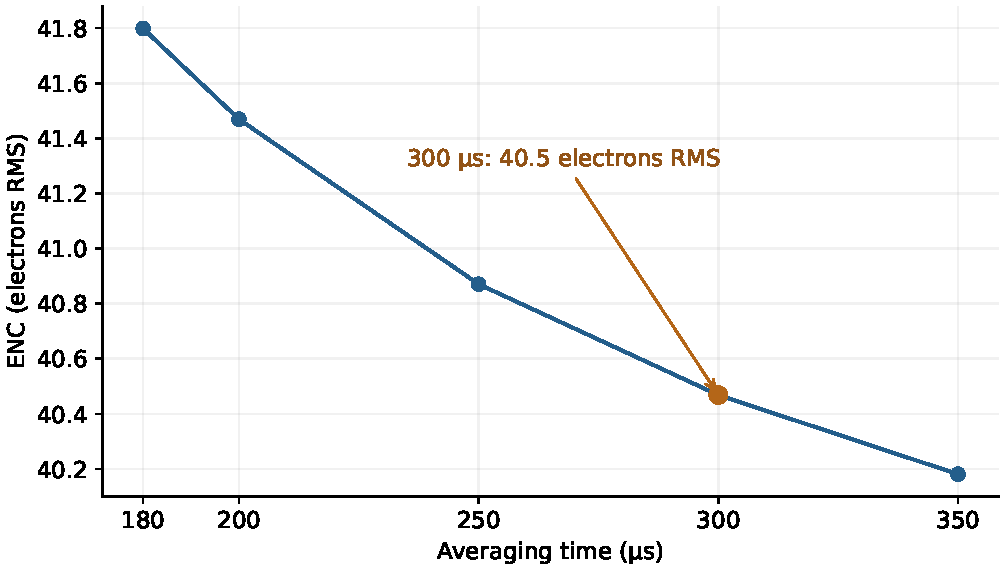
\includegraphics[width=.9\linewidth]{spice_averaging.pdf}
\begin{tabular}{rrrr}\toprule
Average ($\mu$s) & Gain ($\mu$V/ion) & Noise (mV RMS) & ENC ($e$ RMS)\\\midrule
180 & 15.5 & 0.648 & 41.8 \\
200 & 15.49 & 0.643 & 41.47 \\
250 & 15.48 & 0.633 & 40.87 \\
300 & 15.47 & 0.626 & 40.47 \\
350 & 15.46 & 0.621 & 40.18 \\
\bottomrule\end{tabular}
\end{center}
The 300 $\mu$s point reproduces the independent saved Python calculation
within $10^{-9}$ relative tolerance. Checks compare quadrature orders 8 and 16,
noise spectra with 200 and 400 points per decade, and two transient resolutions.
The white-noise integral agrees with the non-overlapping box-average identity
to 0.2\% over the finite integration band.


Maximum relative differences: quadrature relative error: 1.44e-14, spectral relative error: 3.99e-07, transient relative error: 3.09e-07.
\end{document}
